\subsection{Monitoring}
To monitor our systems, Prometheus is used to collect metrics and Grafana is used to visualize them. We chose to monitor the number of requests and request latency for each endpoint on our server, and we monitored the CPU and memory usage of it. We chose these because they give a quick overview of how the system is performing. The remaining information is stored in our logs.

For an example where we had an issue with our system, which was reflected in the monitoring, see \appendixref{appendix:monitoring-samples}.

\begin{figure}[H]
    \makebox[\textwidth][c]{
        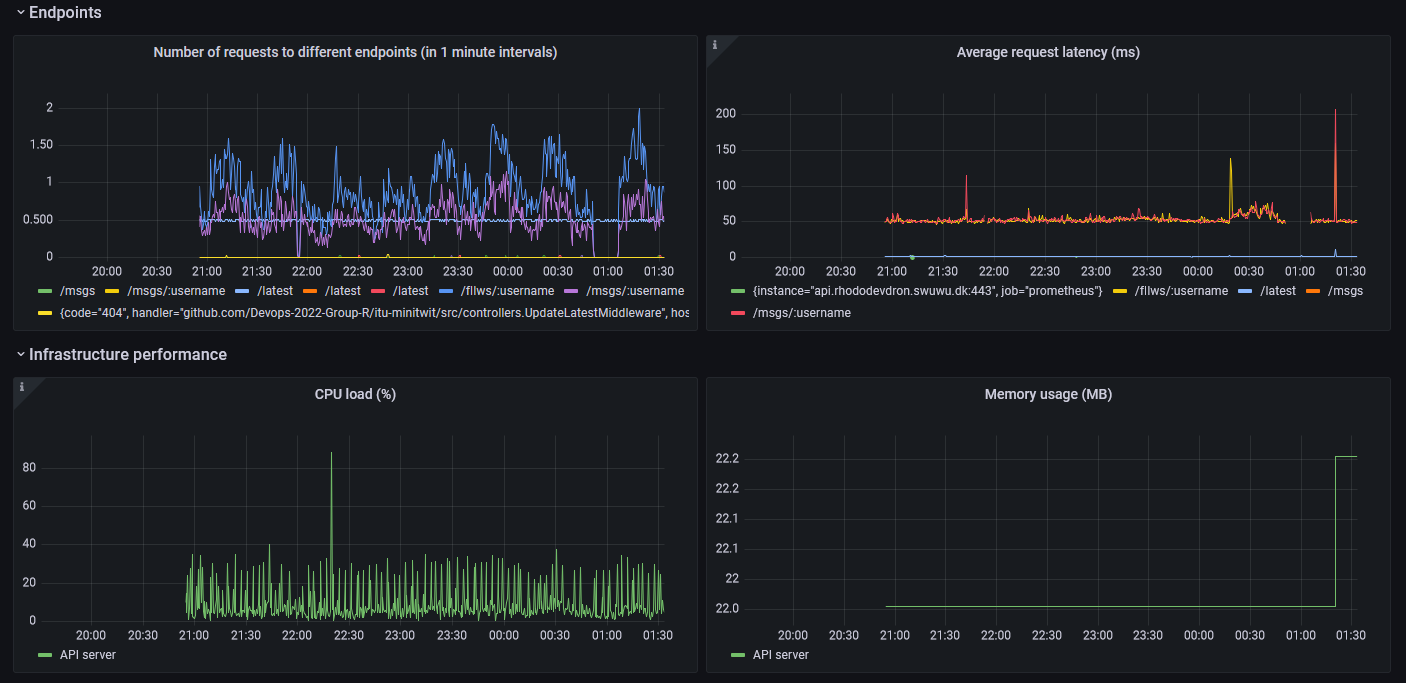
\includegraphics[width=0.85\paperwidth]{grafana-dashboard}
    }%
    \caption{A sample of our Grafana dashboard.}
\end{figure}
